\chapter{Conclusion and Outlook}
\label{chap:conclusion}

\section{Future work}
The developed software still offers potential for future expansion and improvements. For instance, the software misses some of the useful tools that are present in other modeling software such as simple predefined shapes (like cubes or cylinders), mirroring and merging meshes. Using a second VR controller (e.g.\ the Oculus Touch controller) gives enough buttons to map these functions to, allowing us to implement them without the addition of menu, thus staying with the principle of "intuitive" hand gestures. Adding an extra controller also allows for the user to switch between smooth and sharp curve deformation. The functionality for this is embedded in the software, but is not mapped to any button because all buttons of the first controller are already occupied by other functions. 

Another functionality that would prove to be useful in many cases is the possibility to use blueprint images. When working with blueprint images, the user defines a series of different images of an object each taken from a different viewpoint. This allows them to trace these silhouettes from different angles and precisely recreate the object they want to model.

Additionally, the quality of the created meshes could greatly be improved by applying intermediate remeshing. As can be seen from the mesh examples, the triangle sizes differ greatly between triangles that are part of the initial created shape and triangles that are part of a subsequent cut surface or extruded part. This makes the appearance of the mesh rather chaotic and this could be avoided by remeshing every time a new surface is created. The purpose of the remeshing would be to make the edge lengths more uniform across the different parts of the mesh, resulting in a much more homogeneous mesh structure.

Final possibilities for improvements to the software lie in improving the interface. Implementing hand avatars for hand orientation instead of a simple sphere greatly increase the feeling of immersion. Furthermore, displaying the currently selected tool modes (for example cutting versus extrusion mode) is an addition that will greatly help the user in keeping track of the type of mood that is selected, especially when there is a lot of switching going on. This could be done either by including a HUD (head-up display), a distanced billboard or customized meshes for each tool as is done in Google Blocks (Figure ~\ref{fig:blocks_tool} gives an example). Additionally enabling the user to navigate the mesh either with one of the thumbsticks or with hand gestures using the two controllers is a valuable extension that will improve the usability, especially for users who do not have a lot of space available to physically walk around the mesh. 

\begin{figure}[!h]
    \centering
    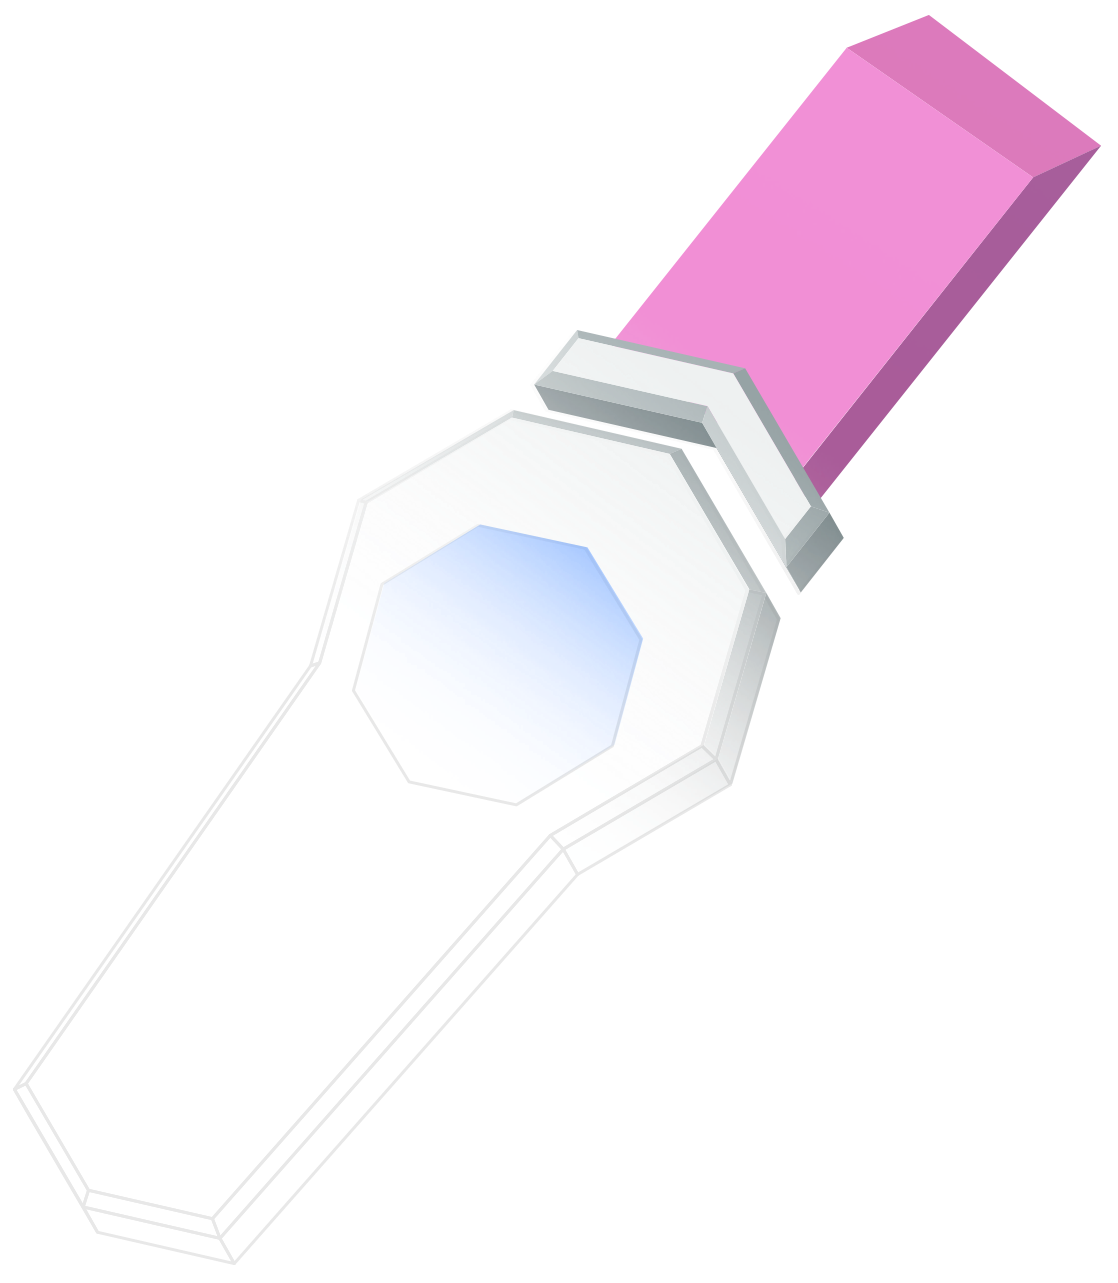
\includegraphics[width=0.3\linewidth]{figures/blocks_tool}\\
    \caption[Google Blocks tool avatars]{Google Blocks' customized hand avatar for the eraser mode.
      \label{fig:blocks_tool}}
\end{figure}

\section{Conclusion}
In this thesis we have presented a novel way of creating 3D models in virtual reality. Modeling 3D objects in VR in itself is not a novel concept, but to the best of our knowledge our software newly introduces the sketch-based 3D modeling paradigm to VR. Whereas other programs mostly work with volumetric brushes and tools to edit the created "clay-like" models, ours transfers the concept of sketch-based modeling to VR by letting the user define model silhouettes. Although volumetric brushes allow for more fine-grained control over the resulting model, we believe that our method provides a more accessible and effortless way of creating simple models. In our opinion, if the goal is to provide the user with an intuitive and uncomplicated way of creating 3D models in VR, SketchMeshVR is better suitable to do the task than other 3D modeling tools for VR like Google Blocks or Oculus Medium. 

We can conclude that virtual reality provides a very useful and powerful extension to traditional 3D modeling and that bringing the sketch-based paradigm to a VR setup makes it even more versatile. Users reported that directly working in 3D especially made out-of-plane editing operations a lot more intuitive as compared to performing these operations in a traditional PC and mouse setting.

The source code for SketchMeshVR (and also its non-VR version), along with instructions for installation can be found online at \url{https://github.com/FloorVerhoeven/SketchMeshVR}. 